% The AIME 2018 bug-on-a-wheel: two concentric circles joined by five
% spokes, with a label at each spoke/circle meeting point and the
% start vertex A marked on the inner circle.
% Source: book/tex/rep-theory/semisimple.tex (Problems) — asy figure.
\documentclass[border=2mm]{standalone}
\usepackage{tikz}
\begin{document}
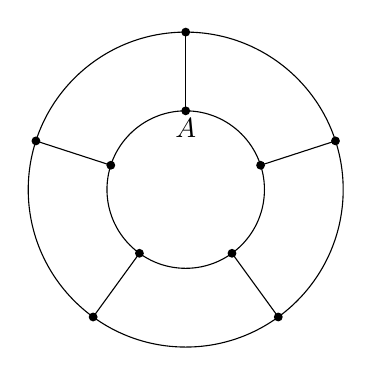
\begin{tikzpicture}
  \draw (0,0) circle (1);
  \draw (0,0) circle (2);
  \foreach \d in {90, 162, 234, 306, 18} {
    \draw (\d:1) -- (\d:2);
    \fill (\d:1) circle (1.6pt);
    \fill (\d:2) circle (1.6pt);
  }
  \node at (90:0.78) {$A$};
\end{tikzpicture}
\end{document}
